\chapter{Einleitung}

Die vorliegende Arbeit widmet sich der Auswertung von Funde und Befunden, die in den 1980er Jahren im nordwestlichen Teil des Kongobeckens gemachten wurden. Sie verfolgt dabei das Ziel, einen Beitrag zur Frage nach Charakter und Verlauf der Besiedlung des zentralafrikanischen Regenwaldes durch keramikproduzierende, sesshaft lebende und Nahrungsmittel anbauende Bevölkerungen zu leisten. Die in dieser Arbeit diskutierten Materialien stammen aus den Prospektions- und Grabungsaktivitäten des unter der Leitung von Manfred K.~H.~Eggert durchgeführten \textit{River Reconnaissance Project}. Der durch das Projekt erstmals archäologisch erschlossene Untersuchungsraum \parencite[siehe][295 Abb.~16.2]{Eggert.1993} kann in zwei Teile untergliedert werden: zum einen das sogenannten \enquote*{Innere Kongobecken}, welches durch die Prospektionen der linksseitigen Zuflüsse des Kongoflusses repräsentiert wird und Gegenstand einer bis in die Anfänge der 1990er Jahre andauernden Auswertungs- und Publikationstätigkeit war \parencites{Eggert.1980b}{Eggert.1981}{Eggert.1983}{Eggert.1984}{Eggert.1984b}{Eggert.1987}{Wotzka.1995}, sowie das Arbeitsgebiet der vorliegenden Arbeit, das \enquote*{nordwestliche Kongobecken}.\footnote{Die hier präsentierte Untersuchung der entlang der rechtsseitigen Zuflüsse des Kongo entdeckten Befunde und Funde orientiert sich, vor allem mit Blick auf die Vergleichbarkeit der gewonnen Erkenntnisse, an der das Innere Kongobecken behandelnden Untersuchung durch Hans-Peter \textcite{Wotzka.1995}.} Dieses, die rechtsseitigen Zuflüsse des Kongo umfassende Gebiet und sein archäologisches Potential waren bislang lediglich Gegenstand einiger Vorberichte \parencites{Eggert.1987c}{Eggert.1992}{Eggert.1993}. 

Zur Erarbeitung des räumlich-zeitlichen Bezugssystems wurde die aus dem Arbeitsgebiet vorliegende Gefäßkeramik herangezogen. Sie eignet sich für eine strukturellen Praxisvergleich vor allem aufgrund ihrer Präsenz im Alltag der zu untersuchenden Gesellschaften sowie der Tatsache, dass sie aufgrund ihrer Kontinuität einen diachronen Vergleich erlaubt \parencite[86]{Saev.2015}. Ausgangspunkt bildeten dabei die Inventare von insgesamt 19 ausgegrabenen oder hinreichend archäologisch untersuchten Befunden (Katalog~A). Sie wurden um Inventare ergänzt, die bei Surveys innerhalb der modernen Dörfer erschlossen wurden (Katalog B). Die Untersuchung der Quellen (Kap.~\ref{sec:Quellen}) vollzieht sich auf zwei Ebenen: auf die Auseinandersetzung mit Indizien zur Keramiktechnologie (Kap.~\ref{sec:Herstellung}) folgt eine detaillierte Beschreibung von auf stilistischem Wege erarbeiteten keramischen Gruppen, im weiteren \enquote*{Stilgruppen} genannt (Kap.~\ref{sec:Keramiksequenz}). Sie bilden die grundlegende Entität für die Rekonstruktion der Besiedlungsgeschichte des Arbeitsgebietes (Kap.~\ref{sec:BesiedlGesch}).

Rückschlüsse auf den Charakter sowie den Verlauf der Besiedlung des Kongobeckens durch keramikproduzierende, sesshaft lebende und Nahrungsmittel anbauende Gruppen lassen sich zum gegenwärtigen Zeitpunkt lediglich auf Grundlage einer sehr eingeschränkten Quellenbasis ziehen. Ausschließlich im Rahmen des \textit{River Reconnaissance Project} wurden bisher systematisch Prospektionen sowie Grabungen durchgeführt. Grundlegende archäologische Sequenzen liegen lediglich für ausgewählte Regionen vor \parencites{Wotzka.1995}{MbidaMindzie.19951996}{AssokoNdong.20002001}{Clist.20042005}{Lavachery.2010}. Weite Teile Zentralafrikas\footnote{Unter \enquote*{Zentralafrika} wird im Sinne dieser Arbeit das Staatsgebiet Äquatorialguineas, Gabuns, Kameruns, der Demokratische Republik Kongo (Kongo-Kinshasa), der Republik Kongo (Kongo-Brazzaville) und der Zentralafrikanischen Republik sowie der nördliche Teil Angolas verstanden \parencite{Eggert.2014}. Verschiedentlich werden auch noch der Süden des Tschads sowie Ruanda und Burundi zu diesem Raum hinzu gezählt \parencite{Maret.2005}.} sind bis heute archäologische \textit{terra incognita}.

\section{Arbeitsgebiet und Fragestellung}\label{sec:Arbeitsgebiet}

Unter der Bezeichnung \enquote*{nordwestliches Kongobecken} werden in dieser Arbeit die 1985 und 1987 durch das \textit{River Reconnaissance Project} befahrenen Flussabschnitte des Sangha, Ngoko, Likwala-aux-Herbes, Ubangi und Lua sowie ein kurzes verbindendes Stück entlang des Kongo zwischen der Ubangi- und Sangha-Mündung verstanden (Abb.~\ref{fig:ArbeitsgebietKarte}). Das eigentliche Arbeitsgebiet umfasst administrativ vor allem den nordöstlichen Teil der Republik Kongo (Kongo-Brazzaville) sowie unmittelbar angrenzende Regionen Kameruns, der Zentralafrikanischen Republik sowie der Demokratischen Republik Kongo (Kongo-Kinshasa). Im nördlichen Teil, entlang des oberen Ubangi, deckt das Arbeitsgebiet die Grenzen der heutigen Provinzen Süd-Ubangi sowie Nord-Ubangi ab.

% in [] Angaben zur Positionieurng des Grafikrahmens h = here; t = top, p = this page
\begin{figure*}[p]
	\centering
	% \includegraphics[width=\textwidth]{output/figs/1_Fundstellen_GIS.pdf}
	\includegraphics[width=.95\textwidth]{fig/1_Fundstellen.pdf}
	\caption{Arbeitsgebiet: Untersuchte Fundstellen. \\ Study Area: ... . \\ Region de etude: ... .}
	\label{fig:ArbeitsgebietKarte}
\end{figure*}

Das Arbeitsgebiet beschreibt einen Nord–Süd-Transekt von der Feuchtsavanne nördlich von Bangui (Zentralafrikanische Republik) bis in den äquatorialen Regenwald südlich von Mba\-ndaka (Demokratische Republik Kongo). In Nord--Süd-Richtung erstreckt es sich über 700\,km, während es in Ost--West-Richtung annähernd 500\,km groß ist. Alle Fundstellen liegen zwischen 289--390\,m\,ü.\,NN.\footnote{Die Höhen der Fundstellen wurden einem SRTMv3-Datensatz mit einer Grundauflösung von 3 Bogensekunden beziehungsweise etwa 90\,m entnommen (Quelle NASA/USGS; \url{https://earthexplorer.usgs.gov} Zugriff: 04.10.2014).}

\begin{table*}[t]
\centering
{\small \begin{tabular}{@{}p{.2\textwidth}R{.11\textwidth}p{.5\textwidth}@{}}
\toprule
\textbf{Flusslauf} & \textbf{Befahrung} & \textbf{Endpunkt} \\
\midrule
Ubangi & 850\,km & Kouango (Fpl.~229) \\
Lua & 97\,km & Fulu-Kaba (Fpl.~233) \\
Kongo/Za{\"i}re & 60\,km & Zwischen Gombe (Fpl.~234) und Lokolela (Fpl.~237) \\
Sangha & 597\,km & Bomasa (Fpl.~274a) \\
Ngoko & ca. 80\,km & Yengo (Fpl.~282)\\
Likwala-aux-Herbes & 526\,km & Matoko (Fpl.~307) \\
\bottomrule
\end{tabular}}
\caption{Arbeitsgebiet: Prospektierte Flussabschnitte (siehe Abb.~\ref{fig:ArbeitsgebietKarte}).}
\label{tab:ArbeitsgebietFlussstrecken}
\end{table*}

Die Feldarbeiten des \textit{River Reconnaissance Project} in der zweiten Hälfte der Kampagne von 1985 sowie während der Kampagne von 1987 deckten etwa 2130\,km der Flussläufe des Ubangi, Lua, Sangha, Ngoko und Likwala-aux-Herbes ab (Tab.~\ref{tab:ArbeitsgebietFlussstrecken}). Ausgehend von seiner Mündung in den Sangha, die etwa 3\,km nördlich von Ouesso (Fpl.~265) liegt, wurde der Ngoko auf einer Strecke von etwa 80\,km stromauf befahren.\footnote{Der untere Abschnitt des Dja, der in Kamerun entspringt, wird ab dem Punkt, an dem er die Grenze zwischen Kamerun und der Republik Kongo bildet (2$^\circ$12$'$25$''$~N, 14$^\circ$35$'$42$''$~O) als \enquote*{Ngoko} bezeichnet. In Yengo (Fpl.~282) musste die Prospektion aufgrund der Malaria-Erkrankung eines Mitarbeiters vorzeitig beendet werden.\label{ftn:DjaNgoko}} Der Sangha bildet den Unterlauf des Kadeï, der in Nordkamerun nahe Garoua-Bouleï entspringt und ab Nola (Zentralafrikanische Republik) als Sangha bezeichnet wird. Der Fluss mündet bei Mossaka, etwa 220\,km südwestlich von Mbandaka, in den Kongo. Er wurde auf einer Länge von fast 600\,km bis an das Dreiländereck der Republik Kongo, Kamerun und der Zentralafrikanischen Republik, knapp nördlich von Bomasa (Fpl.~274a) befahren. Zwischen den Flüssen Sangha und Ubangi liegt der Likwala-aux-Herbes, der auch als Likwala-Esobe oder Likouala-aux-Herbes bezeichnet wird und nordwestlich des Lac Tele entspringt. Der Likwala-aux-Herbes wurde insgesamt auf einer Strecke von über 500\,km befahren, bis zur nicht passierbaren Brücke bei Matoko (Fpl.~307).\footnote{Der Fluss darf nicht mit dem Likwala-Mossaka verwechselt werden, der auf einigen Karten nur mit der Bezeichnung \enquote*{Likwala} verzeichnet ist. Er verläuft westlich des Sangha und mündet bei Mossaka, wie auch der Sangha, in den Kongo.} Der Ubangi zählt zu den größten Zuflüsse des Kongo und bildet in seinem Nordwesten, die Grenze zwischen der Demokratischen Republik Kongo und der Zentralafrikanischen Republik sowie der Republik Kongo. Er entspringt aus dem Zusammenfluss von Uele und Mbomou bei Yakoma (Demokratische Republik Kongo) und mündet etwa 90\,km südwestlich von Mbandaka in den Kongo. Der Ubangi wurde auf einer Strecke von etwa 850\,km, bis Kouango (Fpl.~229) befahren. Der Lua ist neben dem Ngiri einer der größten linksseitigen Zuflüsse des Ubangi. Er mündet bei Dongo (Fpl.~202), etwa auf halber Strecke zwischen Impfondo und Libenge (Fpl.~208), in den Ubangi und wurde auf einer Strecke von etwa 100\,km bis Fulu-Kaba (Fpl.~233) prospektiert.

\vspace{1.5em}
\noindent Basierend auf diesen Feldarbeiten der 1980er Jahre ließen sich für die in dieser Arbeit präsentierte Erstbearbeitung der Befunde und Funde aus dem nordwestlichen Kongobecken eine Reihe von Fragestellungen und Arbeitszielen formulieren:
\begin{itemize*}
\renewcommand\labelitemi{--}
\item Die Auswertung der ausgegrabenen Befunde in Maluba (Fpl.~230; Kat.-Nr.~1--5) , Bobusa (Fpl.~239; Kat.-Nr.~6--7), Pikunda (Fpl.~255; Kat.-Nr.~8--10), Boleko (Fpl.~285; Kat.-Nr.~14) und Munda (Fpl.~304; Kat.-Nr.15--18).
\item Die Aufnahme und Auswertung der noch nicht bearbeiten Keramik des \textit{River Reconnaissance Projects} aus den Feldkampagnen von 1985 (Flüsse: Ubangi und Lua) und 1987 (Flüsse: Sangha, Ngoko und Likwala-aux-Herbes).
\item Die Formulierung einer Besiedlungsabfolge für die befahrenen Flussläufe des Sangha/Ngoko, Likwala-aux-Herbes und Ubangi/Lua.
\item Ein Vergleich der erarbeiteten archäologischen Sequenz mit benachbarten Regionen, allen voran dem von \textcite{Wotzka.1995} untersuchten Inneren Kongobecken.
\end{itemize*}

\noindent Aus diesen Hauptzielen ergaben sich eine Reihe von Kernfragen:
\begin{itemize*}
\renewcommand\labelitemi{--}
\item Welche keramischen Stilgruppe lassen vor dem Hintergrund der beobachtbaren Variabilität keramischer Formen im Arbeitsgebiet formulieren?
\item Welche Rückschlüsse auf Herstellungstechniken lassen sich an den beobachteten technischen Eigenschaften der Gefäßkeramik ableiten?
\item Welches sind die ältesten im Arbeitsgebiet anzutreffenden keramischen Stilgruppen?
\item Welche relativ- sowie absolutchronologischen Verbindungen bestehen zwischen den einzelnen keramischen Stilgruppen des Arbeitsgebietes?
\item Welche Beziehungen bestehen zwischen den keramischen Stilgruppen des nordwestlichen Kongobeckens und denen der umgebenden Regionen, vor allem dem Inneren Kongobecken?
\item Welche keramischen Stilgruppen des Inneren Kongobeckens können auch im nordwestlichen Kongobecken beobachtet werden?
\item Welche Konsequenzen ergeben sich aus den neu hinzugewonnene Erkenntnissen aus der Sequenz des nordwestlichen Kongobeckens für die Besiedlungsgeschichte des Kongobeckens allgemein?
\item Welche Anpassungen an den Lebensraum \enquote*{Regenwald} lassen sich aus der Besiedlungsabfolge und neueren Paläoumweltdaten ableiten?
\item Welche Auswirkungen haben diese neuen Erkenntnisse auf den Themenkomplex \enquote*{Bantu-Expansion} und die verschiedenen diskutierten Hypothesen und Modelle?
\end{itemize*}

%\noindent Die vorliegende Arbeit zielt folglich nicht auf eine reine, erste Bestandsaufnahme des keramischen Materials, deren Gliederung in Stilgruppen und eine Zusammenfassung zu einer keramischen Sequenz ab, sondern verfolgt auch über das eigene Arbeitsgebiet hinaus reichende Fragenkomplexe.

\section{Forschungsgeschichte}

\subsection*{Feldforschung vor 1977}

Die Geschichte der archäologischen Erforschung des Kongobeckens bis in die späten 1980er Jahre, mit besonderem Fokus auf das Innere Kongobecken, wurde durch Hans-Peter \textsc{Wotzka} (ebd. 22--31) systematisch vorgestellt. Der benachbarte nordwestliche Teil des Kongobeckens muss wie weite Teile des zentralafrikanischen Regenwaldes als eine archäologisch unterrepräsentierte Region gelten. Die erste archäologische Ausgrabung im Arbeitsgebiet wurde 1968 durch Roger de \textcite{deBayledesHermens.1975} durchgeführt. Er legte einen kleinen Testschnitt von 6\,m\textsuperscript{2} (2\,\( \times \)\,3\,m) in Batalimo am linken Ufer des Lobaye (Abb.~\ref{fig:BTM-Verbreitung}) an, einem Zufluss des Ubangi (ebd. 206--221). In einer Kulturschicht kamen umfangreiche Mengen Keramik sowie Steinartefakte zu Tage. Bereits bei der Grabung konnten zwei keramische Gruppen unterschieden werden: flachbodige, reich verzierte Gefäße und einfache, unverzierte Töpfe mit sich leicht verengender Öffnung \parencites[224ff., 234]{Aumassip.1975}[134]{Eggert.1987c}. Eine dem reich verzierten Material aus Batalimo entsprechende Keramik wurde 1985 auch von \textsc{Eggert} (ebd. 137--141) an der Fundstelle Maluba am Lua (Fpl.~230) entdeckt und in Zusammenschau mit den älteren Funde vom Lobaye unter der Bezeichnug \enquote*{Batalimo-Maluba-Gruppe} subsumiert (siehe Kap.~\ref{sec:BTM-Gr}).

Zwischen Dezember 1972 und März 1973 untersuchte Francis Van Noten in Motenge-Boma am Ubangi (Fpl.~206) eine oberflächlich sichtbare Fundkonzentration von geschliffenen Steinbeilen. Eine kleine Grabung mit einigen Testschnitten erbrachte aber nur wenig rouletteverzierte und vom Ausgräber in der Folge als \enquote*{eisenzeitlich} angesprochene Keramik \parencite[58]{vanNoten.1982}. Die in den Testschnitten erfasste Gruben enthielten wenig Material und reichten nicht sehr tief, was von van Noten als Indiz eines jungen Alters gedeutet wurde (ebd.~69). Die Keramik wird von ihm mit Formen aus weiter nördlich gelegenen Regionen in Verbindung gebracht, soll aber auch Merkmale der zeitgenössischen, lokalen Keramik zeigen. So würden moderne, hölzerne Schnitzroulettes eine ähnliche Verzierung hervorbringen, wie sie auf den ausgegrabenen Stücken zu sehen sind (ebd.). Eine detaillierte Vorlage der von Van Noten am Fundplatz Motenge-Boma durchgeführten archäologischen Maßnahmen liegt nicht vor, so dass sich über die geschilderten Sachverhalte hinaus, keine Angaben machen lassen. Funde, die der von Van Noten präsentierten Keramik (ebd. Abb.~40; siehe Abb.~\ref{fig:MotengeBoma_VanNoten_Keramik}) entsprechen wurden auch im ausgewerteten Fundmaterial erfasst und unter der Bezeichnung \enquote*{Motenge-Boma-Gruppe} systematisiert (siehe Kap.~\ref{sec:MTB-Gr}).


\subsection*{Feldforschung des \textit{River Reconnaissance Project} (1977--1987)}

Der archäologische Forschungsstand im Kongobecken geht fast ausschließlich auf das von der Deutsche Forschungsgemeinschaft geförderte und von Manfred K.~H. Eggert geleitete Regen"-wald-Projekt zurück. Von September 1977 bis Februar 1978 wurden im Rahmen eines ersten Aufenthalts im Ruki-Gebiet, östlich der Provinzhaupstadt Mbandaka erstmals systematisch archäologische Arbeiten in der Äquatorregion der Demokratischen Republik Kongo (ehem. Zaïre) durchgeführt \parencites[407--426]{Eggert.1980b}[23f.]{Wotzka.1995}. Das im Anschluss, ebenfalls durch die DFG geförderte, \textit{River Reconnaissance Project} lief von 1981--1987. Insgesamt wurden fünf jeweils sechsmonatige Feldaufenthalte mit großräumigen ethnologischen und archäologischen Surveys und Grabungen in der Demokratischen Republik Kongo, der Republik Kongo (ehem. Volksrepublik Kongo) sowie angrenzenden Regionen (Zentralafrikanische Republik und Kamerun) unternommen. Das Projekt hatte die Untersuchung der Archäologie der großen Zuflüsse des Kongo-Stroms zum Ziel und zusammengenommen wurden etwa 5000 Flusskilometer befahren \parencite[295]{Eggert.1993}.

Der bisherige Stand der Ergebnisse des Projekts liegen in Forme einer umfangreichen Anzahl von Vorberichten \parencites{Eggert.1980b}{Eggert.1981}{Eggert.1983}{Eggert.1984}{Eggert.1984b}{Eggert.1987}{Eggert.1987c}{Eggert.1992}{Eggert.1993} sowie der Dissertation von H.-P.~\textcite{Wotzka.1995} über die Besiedlung des Inneren Kongobeckens vor. Anhand einer über \enquote{stilistische Bindeglieder geknüpften Kette} erarbeitet \textsc{Wotzka} (ebd. 65) eine umfassende Keramiksequenz für die linksseitigen Nebenflüsse des Kongo-Stromes erstellt. Die Besiedlungsgeschichte der einzelnen Flussgebiete und letztlich des gesamten Inneren Kongobeckens werden für die vergangenen 2400 Jahre mit archäologischen Methoden nachgezeichnet und ihre Relevanz im Kontext der Bantu-Expansion erörtert.

Die sogenannte Imbonga-Keramik bildet dabei den frühesten Keramikstil im Inneren Kongobecken (ebd. 65). Die derzeit vorliegenden absoluten Datierungen für den Imbonga-Stil fallen ungefähr in den Zeitraum zwischen 400--100~v.~Chr. (ebd. 67). Woher die Menschen gekommen waren, die vor knapp zweieinhalb Jahrtausenden Imbonga-Keramik herstellten und die Äquatorregion der heutigen Demokratischen Republik Kongo besiedelten, ist bis heute ungeklärt, da sich bislang keine direkten Vorläuferstile fanden. Wotzka war jedoch in der Lage, ausgehend von der Imbonga-Gruppe eine stilistische Abfolge bis zu den rezenten Keramikgruppen der Region zu erarbeiten.

Erst die zweite Hälfte der Kampagne von 1985 führte mit der Prospektion des Ubangi aus dem Inneren Kongobecken hinaus. Neben der Prospektion der Flussläufe des Ikelemba (300\,km), des Luolonga (180\,km), des Lopori (180\,km) und des Maringa (545\,km) konnte der Ubangi auf einer Länge von 800\,km sowie der Lua auf 100\,km Länge prospektiert werden \parencite[129]{Eggert.1987c}.\footnote{Keramik ähnlich jener aus Batalimo \parencites{deBayledesHermens.1975}{Aumassip.1975} wurde bei dieser Prospektion an einer Reihe von Fundstellen entdeckt \parencite[134 Fig.~4]{Eggert.1987c}. Vor allem ein in Dongo am mittleren Ubangi (Fpl.~202) gefundener Komplex erbrachte eine größer Anzahl entsprechender Gefäße (Taf.~9.1--5).} In Maluba am unteren Lua (Fpl.~230) wurden mehrere Gruben entdeckt und ausgegraben (Kat.-Nr.~1--5). Sie enthielten ebenfalls Funde mit starker Ähnlichkeit zur Keramik aus Batalimo, die daraufhin von Eggert als \enquote*{Batalimo-Maluba-Horizont} zusammengefasst wurde (ebd. 138--140).

Die Frage nach den Zusammenhängen zwischen der Keramik aus Batalimo und Maluba mit der aus Imbonga konnte auf Basis der 1985 vorliegenden Daten nicht gelöst werden (ebd. 141ff.). Daher wurde das Untersuchungsgebiet des Projekts nach Westen auf das Gebiet der Republik Kongo und Kamerun erweitert. 1987 fanden dann die Prospektionen entlang der Flüsse Sangha und Likwala-aux-Herbes sowie entlang des Ngoko, dem Grenzfluss zwischen der Republik Kongo und Kamerun, statt. Die Flussgebiete des Sangha/Ngoko und Likwala-aux-Herbes waren bis zur Feldkampagne von 1987 archäologische \textit{terra incognita}. Der Survey erbrachte eine Gruppe charakteristischer Keramikgefäße, die nach den beiden wichtigsten Fundstellen von \textcite[16f.]{Eggert.1992} als \enquote*{Pikunda-Munda-Horizont} bezeichnet wurde.

Ein Charakteristikum der Besiedlungsabfolge des nordwestlichen Kongobeckens trat bereits während der Feldarbeiten offen zu Tage: Keramik der frühesten Gruppe des Innere Kongobeckens, der Imbonga-Gruppe, konnte in signifikantem Maße an keiner Fundstelle beobachtet werden \parencite[4; siehe Kap.~\ref{sec:IMB-Gr}]{Eggert.1987c}. Dies warf die Fragen auf, mit welcher Keramikgruppe die Sequenz im nordwestlichen Kongobecken beginnt, woher diese Keramik stammt und ob es Verbindungen zur Imbonga-Keramik des Inneren Kongobeckens gibt. Es wurde indessen bereits deutlich, dass die ursprüngliche Besiedlung nicht vom nordwestlichen Kongobecken aus in das Innere Kongobecken hinein erfolgte, sondern dass die Herkunft der Imbonga-Keramik auf anderen Wegen herzuleiten sei \parencite[257 Anm.~49]{Wotzka.1995}.


\subsection*{Wissenschaftliche Auswertung der Feldarbeiten des \textit{River Reconnaissance Project} (1987--2012)}

Die Auswertung des Fundmaterials aus dem Inneren Kongobecken wurde 1990 durch Hans-Peter Wotzka als Promotionschrift an der Universität Hamburg vorgelegt und 1995 veröffentlicht. Die Arbeit Wotzkas umfasst die Auswertung der Befunde und Funde aus den Feldaufenthalten von 1977 bis 1985 im Gebiet der linksseitigen Zuflüsse des Kongo, dem Inneren Kongobecken. Ausgenommen war die Auswertung von Verhüttungsbefunden aus Bamanya am Ruki (Fpl.~12) sowie Grabungen im Bereich eines Grabenwerkes in Mondjo am Ikelemba (Fpl.~133).\footnote{Mit der Vorlage der vorliegenden Arbeit sind die beiden großen Materialblöcke des \textit{River Reconnaissance Project} ausgewertet und vorgelegt. Im Rahmen dieser Arbeit bliebt die Auswertung der Befunde aus Bamanya (\textsc{Wotzka} 1995: Fpl.~12) und Mondjo (ebd. Fpl.~133) ebenfalls offen. Das Fundgut beider Fundstellen war Teil der Auswertungen Wotzkas.} Die Materialien aus der zweiten Hälfte der Feldkampagne von 1985 sowie jenes von 1987 blieben in Wotzkas Auswertung grundsätzlich unberücksichtigt. Er konnte die Funde allerdings in Augenschein nehmen und in Form kurzer Verweise auf Details eingehen (ebd. 29, 68, 107, 119, 139, 270--272).

Die Funde aus dem nordwestlichen Kongobecken, das 1985 sowie 1987 erschlossen wurde, wurden -- noch in Hamburg -- beschriftet und in einer umfangreichen Auswahl gezeichnet. Eine zweite Auswahl Keramik wurde, nach der Berufung des Projektleiters M.~K.~H. Eggert als Professor nach Erlangen und später Tübingen an letztgenanntem Standort Ende der 1990er Jahre\footnote{Diese Arbeiten wurden von Almuth Mehling, Stefanie Samida und Michele Williams-Schmitt durchgeführt.} in einer kombinierten Methode aus gezeichnetem Profil und Fotografie der Ansichten als Tafelabbildungen vorbereitet. Mehrere originale Fundzeichnungen, die Eingang in einen Aufsatz von \textcite{Eggert.1993} fanden, wurden nach der Drucklegung des Manuskripts nicht mehr zurückgesandt.

Bis zum Ende der 1990er Jahre, als die Aufarbeitung der Materialien unterbrochen wurde, waren die folgenden Arbeitsschritte der wissenschaftlichen Auswertung in verschiedenen Stadien der Bearbeitung:
\begin{itemize*}
\renewcommand\labelitemi{--}
\item Hermann Holsten war mit der Sortierung und Beschriftung der Funde sowie einer Kurzcharakterisierung aller angetroffenen keramischen Komplexe betraut.
\item Célestin Kanimba Misago fertigte 1995 eine einseitige Kurzbeschreibung des 1987 in Pikunda am Sangha (Fpl.~255) von ihm ausgegrabenen Verhüttungysbefundes PIK 87/3 an (Kat.-Nr.~10; \textsc{Kanimba-Misago} 1995). Aufgrund es Fehlens der originalen Dokumentation stellt dieser Text die einzige vom Ausgräber stammende Beschreibung des Befundes dar.
\item Holsten und Frank Nikulka waren mit einer ersten Auswertung der Grabung in Munda (Fpl. 304) betraut und sind die maßgeblichen Autoren eines diesbezüglichen Manuskriptes.
\item Kanimba Misago und Thomas Knopf arbeiteten bis Ende der 1990er Jahr an einer systematischen Erfassung der formalen Eigenschaften sowie der Verzierungselemente der Keramik aus dem nordwestlichen Kongobecken. Eine erste Arbeitsgliederung der beabsichtigten Veröffentlichung umfasst eine Gliederung sowie die Bearbeiter der einzelnen Teilaspekte.
\end{itemize*}

\noindent Die Wiederaufnahme der Arbeiten erfolgte 2011. Der Verfasser begann im Rahmen einer Tätigkeit als wissenschaftliche Hilfskraft mit der Sichtung der Materialien. Die ersten Arbeiten umfassten neben der Durchsicht der vorhandenen Aktenlage auch die Inventarisierung und Sortierung des über mehrere Räume verteilten Fundgutes.%Die Quellen waren auf mehrere Büroräume verteilt und wurden mit Unterstützung einer studentischen Hilfskraft geordnet und nach Fundplätzen und Befunden sortiert, neu verpackt und zugleich inventarisiert.

\subsection*{Feldforschung nach 1987}

Zwischen dem Ende der Feldarbeiten des \textit{River Reconnaissance Project} im Jahr 1987 bis zum Beginn der 2010er Jahr erfolgte im Arbeitsgebiet aufgrund politischer Instabilitäten und damit verbundener prekärer Sicherheitslage praktisch keine archäologische Feldforschung. Die Feldarbeiten des \textit{River Reconnaissance Project} fanden Ende der 1990er Jahre ihre Fortführung im Südosten der Republik Kamerun \parencite{Eggert.2002}.\footnote{Die Ergebnisse dieser Feldarbeiten sind bislang nicht umfänglich aufgearbeitet und vorgelegt.}

Im Südwesten der Zentralafrikanischen Republik, vor allem aber der Region um die Hauptstadt Bangui, wurden seit den 1990er Jahren verschiedentlich archäologische Fundstellen neu erschlossen. Vornehmlich handelt es sich um Prospektionsaktivitäten die vor ethnoarchäologischen Fragestellungen durchgeführt wurden und im Rahmen von Qualifikationsschriften an der Universität von Bangui \parencites{Ndanga.199596}{Abrou.199697} oder in Frankreich \parencites{Kote.1992}{Scouflaire.1997} ausgewertet wurden. Die Arbeiten lieferten zwar durchaus neue Datierungen, fanden aber nur selten Eingang in überregionale Synthesen zur Besiedlungsabfolge. Weitere Arbeiten widmeten sich der Metallurgiegeschichte in der Region und verfolgten dabei ebenfalls vornehmlich ethnoarchäologische Forschungsansätze \parencites{Muramira.20042005}{Muramira.20052006}{Moga.2008}. 

In den Jahren 2008 bis 2010 wurden durch Jean-Paul Ndanga neue Grabungen in Batalimo am Lobaye sowie der 1,5\,km entfernt liegenden Fundstelle Ngo Tchororo durchgeführt, die 2010 auch durch Els Cornelissen und Raymond Lanfranchi unterstützt wurden.\footnote{Pers. Mitt. E. Cornelissen (06.10.2016).} Der 2009 durch Nganda angelegt Testschnitt in Batalimo wurde 2010 erweitert \parencite[siehe Kap.~\ref{sec:BTM-Gr}]{Ndanga.2010}.\footnote{Eine systematische Auswertung der Befunde und Funde steht aufgrund der politischen Instabilität innerhalb der Zentralafrikanischen Republik gegenwärtig aus.}

Die seit den 2010er Jahren in der Region durchgeführte Forschungsvorhaben mit internationaler Beteiligung verfolgten häufig paläo-ökologische-archäologische Forschungsansätzen \parencites[siehe][]{Kiahtipes.2011}{Kiahtipes.2016}{Gillet.2013}{MorinRivat.2014}. Im Jahr 2011 wurden durch die Arbeitsgruppe um Karen Lupo ausgedehnte archäologische und paläo-ökologische Prospektionen sowie kleinere Testschnitte im Umfeld des Fundplatz Bagbaya in der südwestlichen Zentralafrikanischen Republik angelegt \parencite{Lupo.2015}.\footnote{Der Ortsname \enquote*{Bagbaya} lässt sich mit \enquote{Eisenmarkt} übersetzen (\textsc{Lupo} 2015: 3). Neben zwei offenen Abbaugruben für Eisenerz wurden 18 etwa 1,5 bis 2\,m hohe sowie 15 flachere in die vorkoloniale Zeit datierende sowie einige ältere Schlackehügel entdeckt (ebd. 6 Tab.~1, 8). Bei den in den beiden untersuchten Abbaugruben gewonnen Erzen handelt es sich um Eisen reiche, vulkanische Ablagerungen (ebd. 6). Insgesamt elf der prospektierten Schlackehügel wurden durch kleine, 1\,$\times$\,1 oder 1\,$\times$\,2\,m große Testschnitte näher untersucht (ebd. 8). Bei den in den Testschnitten gefundenen Schlacken handelt es sich um blasige Fließschlacken, die als primäre Verhüttungsschlacken angesprochen werden (ebd. 10). Die Bedeutung einiger der Schlackehügel als Anzeiger für Eisengewinnung war der lokalen Bevölkerung sehr gut bekannt, wie mündliche Befragungen ergaben (ebd.).} Konkrete Verhüttungsbefunde im Sinne von Öfen wurden nicht erfasst. Die Ausgräber interpretieren ihre Ergebnisse sehr weitreichend als Zeichen eines vorkolonialen, regionalen Handelsnetzes, das bis in die ethnohistorische Zeit reichte (ebd.~2). Zusammen mit den archäologischen Arbeiten wurden paläo-ökologische Untersuchungen durchgeführt.\footnote{Nahe des Zusammenflusses der Flüsse Loame und Lobaye wurde in einer Region mit Feuchtsavannen-Vegetation ein 2\,m langer Sedimentkern erbohrt (\textsc{Lupo} 2015:5). Der Kern wurde mittels eines mobilen \enquote*{russischen PEAT-Bohrers} erbohrt und im Feld im Abstand 5\,cm beprobt. Für weitere Untersuchungen wurden je 1\,cm große Abschnitte entnommen (ebd.). Radiokohlenstoffdatierungen ergaben, dass der Kern Paläoumweltdaten der letzten 500 Jahre umfasst (ebd. 13 Abb.~6). Der Kern deutet einen Wechsel von einer dichten Regenwaldvegetation zu einer offeneren, savannenartigeren Vegetation im späten 17. oder frühen 18.~Jh. an.}

Neben dem Südwesten der Zentralafrikanischen Republik, rückte der Norden der Republik Kongo, auch durch umfangreiche Konzessionen für Holzeinschlag \parencite[siehe][Abb.~S3]{Gond.2013}, und vor allem die Region des Sangha vermehrt in den Fokus der Forschung. Neue Fundstellen und Radiokohlenstoffdatierungen, bislang jedoch keinerlei Angaben zu mit den Funden assoziiertem archäologischen Fundgut, lieferte eine Arbeitsgruppe um Richard \textcites{Oslisly.2013b}{MorinRivat.2014}. Einzig von der am Sangha, etwa 25\,km südöstlich von Ouesso (Fpl.~265) gelegenen Fundstelle Mboua sind einige wenige Keramikformen bekannt \parencite[95 Abb.~31, 114 Abb.~42]{Gillet.2013}. Das Material kann in die im Rahmen der vorliegenden Untersuchung erarbeitete Stilgruppen-Sequenz der Region integriert werden (siehe Kap.~\ref{sec:SequenzSanghaNgoko}).

Auch außerhalb des eigentlichen Arbeitsgebietes setzte erst zu Beginn der 2010er Jahre wieder erste archäologische Feldforschung ein. Die Region entlang des nördlichen Kongobogens, der Mündungsbereich der Flüsse Itimbiri, Aruwimi und Lomami in den Kongo, wurde erstmals 2010 im Rahmen des \enquote*{Boyekoli Ebale Congo}-Projektes durch Wissenschaftler verschiedener Disziplinen des \textit{Musée royal de l'Afrique centrale} in Tervuren -- auch mit Blick auf die Archäologie -- prospektiert \parencite{LivingstoneSmith.2011}.\footnote{Siehe Kap.~\ref{sec:NordCongo} mit Anm.~\ref{ftn:BoyekoliEbaleCongo}.} Insgesamt wurden sechs Fundstellen erschlossen. Bei Grabungen in Bomane-Yangwa am Aruwimi (1$^\circ$16$'$53$''$~N/23$^\circ$44$'$44$''$~O) wurden zwei Gruben näher untersucht. Einer der Befunde enthielt ein umfangreiches keramisches Inventar \parencite[ebd. 13 Abb. 2; ][5 Abb.~3]{LivingstoneSmith.2017}. Die enge, mit einer Vielzahl von Gefäßen verfüllte Grube erinnert dabei sehr an Keramikdeponierungen in Gruben im Inneren Kongobecken \parencite[siehe][256--264]{Wotzka.1993}. Eine sehr ähnlicher Befund wurde auch in Baombi am Lindi (0$^\circ$39$'$50$''$~N/25$^\circ$8$'$44$''$~O) aufgedeckt \parencites[78--79 Abb.~5--6]{Cornelissen.2013}[8 Abb.~10]{LivingstoneSmith.2017}. In der Zusammenschau ergab sich eine aus drei Phasen bestehende keramische Sequenz, deren ältestes Element durch die Keramik der beiden genannte Fundstellen repräsentiert ist und in das 4.~Jh.~v.~Chr. bis 1.~Jh.~n.~Chr. datiert (ebd. 16--19, 17 Abb.~23). Sie ist somit grundsätzlich zeitlich mit der frühesten, durch die Keramik der Imbonga-Gruppe (Kap.~\ref{sec:IMB-Gr}) repräsentierte Besiedlung des Inneren Kongobeckens \parencite[65]{Wotzka.1995}. Die folgende \enquote*{mittlere Keramikphase} datiert vom 1.--6.~Jh.~n.~Chr., während die jüngere Phase zwischen das 8.--17.~Jh.~n.~Chr. datiert. Die Keramik der jüngeren Phase zeichnet sich unter anderem durch die Nutzung von Rouletteverzierungen aus (siehe Kap.~\ref{sec:Zeitscheiben}).

Im Jahr 2010 wurde neue Feldarbeiten im Inneren Kongobecken durch Hans-Peter Wotzka initiiert.\footnote{Vier erste, von der DFG finanzierte Reisen (2010--2012 sowie 2014) dienten der Etablierung von Kontakten vor Ort, insbesondere zum \textit{Institut des Musées Nationaux du Congo} (IMNC) in Kinshasa. Im Verlauf der zweiten Reise, 2011 konnte Wotzka im Umfeld der Provinzhauptstadt Mbandaka eine kleine Grabung durchführen (mündl. Mitt. \textsc{Wotzka} 2012). Dabei wurde vornehmlich eine Keramik der Stilgruppen Bondongo \parencite[128--139]{Wotzka.1995} und Nkile (ebd. 144--150) enthaltende \enquote*{Schicht} untersucht, die sich über eine längere Strecke in einem Steinbruch verfolgen ließ (mündl. Mitt. \textsc{Wotzka} 2012). Die Keramik sowie gewonnene Radiokohlenstoffproben datieren die Schicht in das 11.--15.~Jh.~n.~Chr. Die \enquote*{Schicht} überlagerte eine Grube mit Keramik der Bokele-Gruppe (ebd. 100--104), die ins 1.--2.~Jh.~n.~Chr. datiert. Die aus der \enquote*{Schicht} sowie der Grube gewonnenen \textsuperscript{14}C-Daten lieferten absolutchornologisch Datierungen für die Bokele-Keramik und bestätigen die chronologische Stellung der keramischen Stilgruppen (mündl. Mitt. \textsc{Wotzka} 2012; siehe ebd. 103f., 138, 149f.). Vor allem für die Keramik der Bokele-Gruppe standen Wotzka bei der Abfassung seiner Dissertationsschrift keine vergleichbar guten Datierungen zur Verfügung. Im Zusammenhang mit der Reise von 2012 führte Wotzka eine Bohrprospektion sowie eine kleine Grabung an der Fundstelle Iyonda (Fpl.~8) durch. In dieser Grabung wurde eine Grube der Imbonga-Gruppe (ebd. 59--68) untersucht, die von einem Befund mit Keramik der Bondongo-Gruppe (ebd. 128--139) überlagert wurde (mündl. Mitt. Wotzka 2012). Aus dem Befund gewonnene Botanikproben wurden zur absoluten Datierung herangezogen. Die insgesamt sechs Datierungen weisen eine starke Überlappung auf und stellen die Grube sicher in das 4.--1.~Jh.~v.~Chr. Sie stützen damit die bis dato bekannten Datierungen für Material der Imbonga-Gruppe, die sich lediglich nach einer quellenkritischen Auseinandersetzung und der resultierenden Zurückweisung der Hälfte der ursprünglich mit Imbonga-Funden assoziierten Datierungen aus den 1980er-Jahren in dieses Zeitfenster einfassen ließ \parencite[66f.]{Wotzka.1995}. Eine Veröffentlichung beider Grabungen ist in Vorbereitung.} Im Zuge dieser ersten Anknüpfungen an die Feldarbeiten des von Eggert geleiteten Regenwald-Projektes durch Wotzka wurde auch eine Kiste mit Bodenproben, welche seit 1987 in der Missionsstation in Bamanya, nahe der Provinzhauptstadt Mbandaka, eingelagert gewesen war, nach Deutschland überführt. Das Probenmaterial sowie ein ähnlich umfangreicher Bestand, der in Tübingen eingelagert war, wurde daraufhin archäobotanisch untersucht. Im Ergebnis dieser Untersuchung konnten erstmals archäobotanische Daten für das Innere Kongobecken vorgelegt werden \parencite{Kahlheber.2014}. Unter anderem fanden sich in Proben aus einer Grube in Boso-Njafo am Lulonga (Fpl.~149) Reste von Perlhirse (\textit{Penniseum glaucum}), die in die Imbonga-Zeit datieren. In einer Probe aus der Grube MUN~87/2-1-3 in Munda am Likwala-aus-Herbes (Fpl.~304; Kat.-Nr.~17) fand sich eine gut erhaltener Samen der Raphia-Palme (ebd. 506, 508 Abb.~7). Mit Jahresbeginn 2015 begann unter der Leitung von Wotzka ein von der DFG finanziertes Projekt, welches sich gemeinsam mit einem von Katharina Neumann geleiteten Botanik-Projekt die Erforschung von Paläoumwelt und Subsistenzbasis im Inneren Kongobecken während der Eisenzeit zum Ziel gesetzt hat.\footnote{Im Jahr 2015 wurden zwei Grabungskampagne in Iyonda (Fpl.~8) durchgeführt, wo Wotzka bereits 2012 eine kleine Grabung unternommen hatte. Während im Laufe der Ersten von Februar bis März 2015 laufenden Kampagne zwei etwa gleich große Grabungschnitte untersucht wurden, lag der Fokus der zweiten, von August bis September 2015 laufenden Kampagne in der Untersuchung von in geomagnetischer Prospektion erschlossenen Anomalien. Die Nutzung geophysikalischer Untersuchungsverfahren ist gegenwärtig an keiner anderen Fundstelle im äquatorialen Regenwald Zentralafrikas durchgeführt worden. Die beobachteten Anomalien erwiesen sich regelhaft als archäologisch ansprechbare Befunde. In einer dritten Kampagne, die Anfang 2016 stattfand, wurden unter Feuchtbodenerhaltung zwei Grabungsschnitte an der Fundstelle Bolondo am Tshuapa (Fpl.~96) ausgegraben. Eine Auswertung der im Rahmen des Projektes erschlossenen Befunde, der daraus stammenden Funde sowie genommener Proben steht gegenwärtig noch aus.}

\todo[inline]{Hist. Berichte: siehe Vennetier.1963}
%\input{chapters/4-1_HistBerichte}

\begin{figure*}[p]
	\centering
	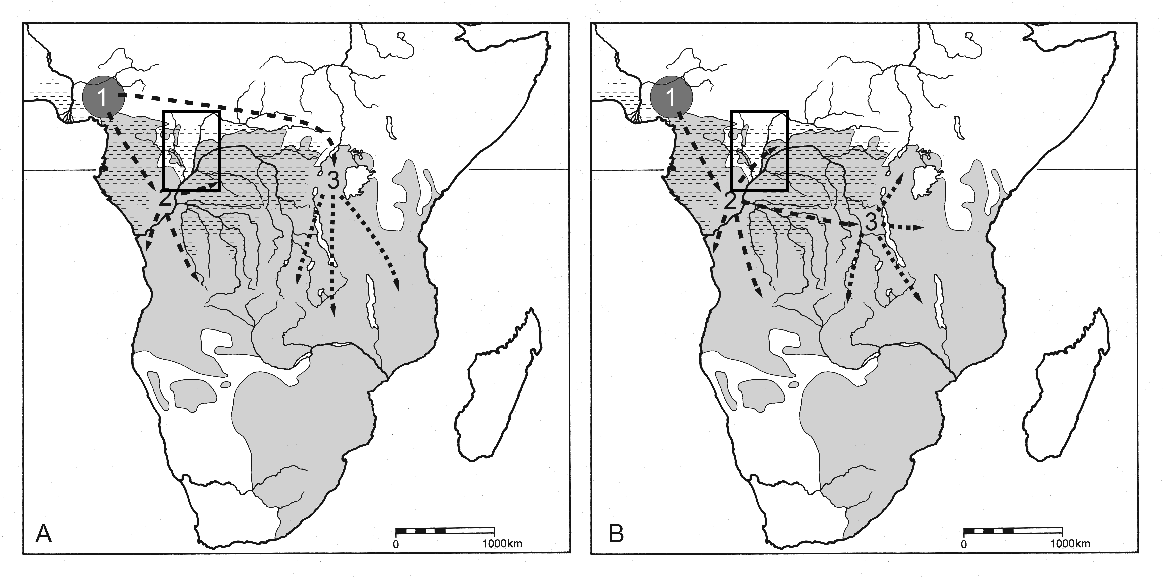
\includegraphics[width=\textwidth]{bib/Eggert2012/207Abb6.pdf}
	\caption{Bantuausbreitung: Gegenwärtig diskutierte Modelle zur Bantuausbreitung und das Arbeitsgebiet \parencites[rot; nach][57, Abb.~2]{Pakendorf.2011}[207 Abb.~6a/b]{Eggert.2012}.}
	\label{fig:Bantuexp_Eggert2012-207Abb6ab}
\end{figure*}


\begin{figure*}[p]
	\centering
	\includegraphics[width=.69\textwidth]{bib/deMaret2013/630Fig43-2.pdf}
	\caption{Bantuausbreitung: Ausbreitungsrouten \parencite[630 Abb. 43.2]{deMaret.2013} und das Arbeitsgebiet (rot).}
	\label{fig:Bantuexp_deMaret2013-630Fig43-2}
\end{figure*}

\section{Archäologie und Historische Linguistik}

Ein zentraler Forschungsgegenstand der Kulturgeschichte Afrikas südlich der Sahara ist die Ausbreitung der Bantu sprechenden Gruppen über fast den gesamten Raum südlich des Äquators: die \enquote*{Bantu-Expansion}. Bantu ist eine Sprachfamilie, der zwischen 300 und 680 einzelne Sprachen zugeordnet werden \parencites{Nurse.2003}[81]{Eggert.2016c}. Die hypothetische Urheimat dieser Sprachfamilie wird derzeit im Grenzgebiet von Kamerun und Nigeria -- im nordwestlichen Eck ihrer heutigen Verbreitung -- verortet (Abb.~\ref{fig:Bantuexp_Eggert2012-207Abb6ab}--\ref{fig:Bantuexp_deMaret2013-630Fig43-2})

Die Frage nach der Ausbreitung der Bantu-Sprachen im südlichen Afrika wurde über Jahrzehnten im Spannungsfeld von Linguistik und Archäologie diskutiert. Die Debatte wies jedoch bereits früh eine starke Vermischung linguistischer und archäologischer Argumente auf, was deutliche Zirkelschlüsse zur Folge hatte \parencites{Eggert.2005}[82]{Eggert.2016c}. Die seit einigen Jahren hinzukommenden Daten aus populationsgenetischen Untersuchungen führten nicht zu einem Aufbrechen dieses Dilemmas. Vielmehr führt die Populationsgenetik zu einer höheren Komplexität und spezifischen Interpretationslücken. So lassen sich auf genetischer Seite nur vertikale Vererbungen von Eltern zu Kindern nachvollziehen, während Sprachgemeinschaften, deren Untersuchung angestrebt ist, auch horizontale Beeinflussungen zulassen \parencite[86]{Eggert.2016c}. Aus diesem Umstand ergibt sich für \textcite{Eggert.2016c} eine Aufweitung des ursprünglichen Dilemmas zu einem Trilemma.

Zur Erklärung der Ausbreitung der Bantu-Sprachen postulieren nicht wenige Forscher mehr oder minder großräumige Wanderungsbewegungen \parencites{Vansina.1995}{Ehret.2001}. Für das Arbeitsgebiet werden eine Reihe linguistisch inspirierter historischer Hypothesen diskutiert \parencite[10f.; siehe Abb.~\ref{fig:Bantuexp_Eggert2012-207Abb6ab}--\ref{fig:Bantuexp_deMaret2013-630Fig43-2}]{Eggert.1992}. So geht \textcite{Ehret.1982} von einer sehr frühen Besiedlung des Regenwaldes durch Bantu-Sprecher aus. Basierend auf Überlegungen von \textcite{Heine.1973} datiert er die frühesten Phasen der Bantu-Expansion in den zentralen Teil des Regenwaldes -- auch in das gesamte Areal westlich des mittleren und unteren Ubangi-Flusses -- bereits an den Beginn des zweiten vorchristlichen Jahrtausends \parencite[58, 63~Karte 10; Abb.~\ref{fig:Bantuexp_deMaret2013-630Fig43-2}]{Ehret.1982}. Für \textcite[51f. Karten~2.7--2.8]{Vansina.1990} hingegen stellten die weiten Sumpfgebiete westlich des Ubangi eine deutliche Barriere für die Ausbreitung der Bantu-Sprecher dar. Er postuliert eine nördliche Ausweichbewegung der allgemein nach Osten gerichteten Ausbreitung des Bantu entlang der nördlichen Grenze des Regenwaldes und lässt die Sangha-Region undatiert (ebd. 51 Karte~2.7; Abb.~\ref{fig:Bantuexp_Eggert2012-207Abb6ab}).

Die Regenwaldgebiete Zentralafrikas sind vor allem deshalb von zentraler Bedeutung für die Annäherung an das Problem der Ausbreitung der Bantusprachen, ja geradezu \enquote{der entscheidende Prüfstein für die Rolle der Archäologie bei der Bantuausbreitung} \parencite[207]{Eggert.2012}, da sie aktuell fast vollständig von Bantu sprechenden Gruppen besiedelt sind und die Aufsiedlung durch keramikherstellende Gruppen im Inneren Kongobecken bereits plausibel mit der Bantu-Ausbreitung verknüpft wurde \parencite[244--246]{Wotzka.1995}. Beim gegenwärtigen Stand der archäologischen Erforschung Zentralafrikas müssen jedoch grundsätzlich alle Versuche, die historische Verbreitung beziehungsweise Ausbreitung kulturell-linguistischer Gruppen zu erfassen, als pure Spekulation bezeichnet werden \parencites[78]{David.1982}[105]{Boyd.2007}. Weder die Historische Linguistik noch die Populationsgenetik sind in der Lage generische Aussagen zur zeitlichen Dimension der jeweils beobachteten Phänomene zu machen \parencite[84]{Eggert.2016c}, dies vermag lediglich die Archäologie.\footnote{Umfassende kritische Auseinandersetzungen zum Spannungsfeld von Historischer Linguistik und Archäologie in der Frage der Bantu-Expansion finden sich bei \textcites{Eggert.2005}{Eggert.2012c}{Eggert.2012}{Eggert.2016c}.}

%\parencite{Bostoen.2015} Sangha-Korridor
%Die Sprachgeschichte des Arbeitsgebietes ... \todo{MEHR}
%>> Grodemund, Rebekka - kritisch würdigen (mündl. HPW 2015)



\section{Geologie und Böden}

Das Arbeitsgebiet umfasst den nordwestlichen Rand des Kongobeckens, jenem intrakontinentalen Becken, das zirka 1,2 Millionen km\textsuperscript{2} groß ist und den Großteil des Kongokratons, einer der vier tektonisch stabilen Schildregionen Afrikas, einnimmt \parencites[16]{Runge.2001}[240]{KadimaKabongo.2011}. Im Kongobecken, auch als \textit{Cuvette central} bezeichnet, ist das präkambrische Grundgebirge von bis zu 3\,km mächtigen, phanerozoischen Sedimentpaketen überlagert. Lediglich in den randlichen Schwellenregionen an der Oberfläche steht es oberflächlich an \parencite[17]{Runge.2001}.\footnote{Diese aus dem Archaikum (4--2,5\,Ma) sowie Paläoproterozoikum (2,5--1,6\,Ma) stammenden Blöcke sind: der \enquote*{Zentral Kasai-Kongo Block} im südlichen Teil der Demokratischen Republik Kongo (DRC) und Nord-/Zentral-Angola, der \enquote*{Kongo-Uganda Block}, der sich vom nordöstlichen der DRC in den Süden der Zentralafrikanischen Republik (RCA) und des Sudans [heute Südsudan] und den Ostens Ugandas reicht sowie der der \enquote*{Kamerun-Gabun-Kongo Block}, der in Kamerun als Ntem-Komplex und in Gabun und der Republik Kongo als Chailu-Block bekannt ist \parencite[240]{KadimaKabongo.2011}.} Die als Hauptwasserscheiden fungierenden, das Kongobecken umgebenden Grundgebirgsschilde bestimmen das zirka 3,7 Million km\textsuperscript{2} große Einzugsgebiet des Kongo, der mit einer mittlere Abflussmenge von etwa 40~000\,m\textsuperscript{3}/s nach dem Amazonas zu den größten Flüssen der Erde zählt \parencite[63]{Runge.2001}.

Die jüngere Geologie des Kongobeckens ist von verlehmten Sanden und weichen Sandsteinen in nahezu horizontaler Schichtung bestimmt \parencite[302, 303 Abb.~2]{Giresse.2005b}, während ein Erosionsereignis am Ende des Tertiär teilweise zur Verlagerung älterer Ablagerungen geführt hat (ebd. 306). Die bislang umfangreichsten Studien zur nachpaleozoischen Geschichte des Kongobeckens \parencites{Daly.1991}{Daly.1992} basieren auf zwischen 1973 und 1981 durchgeführten Geomagnetikprofile und Bohrungen südöstlich von Mbandaka \parencite[301f.]{Giresse.2005b}.

Die in Grundzügen nachvollziehbare geologische Geschichte des Kongobeckens lässt sich wie folgt zusammenfassen (ebd. 313): Die Anhebung der Becken-Ränder am Beginn des Känozoikums beendete eine Phase mariner Einbrüche in ein lakustrin oder lagunal geprägten Milieu. Während des Paläogen bestimmen äoloische Ablagerungen, die \enquote*{Grès Polymorphes Serie} die Becken-Sedimentation. Der Beginn der bis heute andauernden fluvialen Ablagerungsphase im Kongobecken, die mit verstärkter ferralithischer Bodenbildung einhergeht, lässt sich frühestens mit den neogenen Ablagerungen der \enquote*{Sables Ocres Series} in Zusammenhang bringen.

Eine Projektion der Fundstellen auf eine Übersichtskarte der geologischen Grundeinheiten Afrikas \parencite{Persits.2002} erbrachte, das 71\,\% aller bearbeiteten Fundstellen auf holozäne (\enquote*{Qe}), 20\,\% auf präkambrischen Ablagerungen (\enquote*{pCm}), 7\,\% im direkten Fluss-Bereich (\enquote*{H20}) und 2\,\% auf känozoischen Ablagerungen (\enquote*{QT}) zu finden sind. Die Fundstellen im Arbeitsgebiet lassen sich mit Bezug auf den geologischen Untergrund in zwei Gruppen unterteilen: nördlich von Libenge am Ubangi (Fpl.~208) befinden sich die Fundstellen vornehmlich auf präkambrische Formen, während die Fundstellen weiter südlich auf den deutlich jüngeren, känozoischen und holozänen Ablagerungen, welche das gesamte Kongobecken bestimmen, liegen. In nordwestliche Richtung wurde diese geologische Grenze des Kongobeckens mit den Surveys nur knapp überschritten. Lediglich die wenigen Fundstellen am Sangha die flussaufwärts von Gbagbale (Fpl.~270) liegen, befinden sich nicht mehr auf jüngerem, holozänen Untergrund.

Bei den im Arbeitsgebiet angetroffenen Böden handelt es sich zu großen Teilen um Ferralsole. Diese, auch als Oxisole bezeichnete Form der Bodenbildung, zeichnet sich durch eine charakteristische, auf Goethit hinweisende, gelblich bis leicht rötlichen Färbung des Unterbodens aus \parencites[351f., 355 Abb.~7.6-4]{Scheffer.2010}[144]{Jones.2013}. Dieser wird lediglich von einem dünnen, dunklen und humus-reichen Oberboden überdeckt. Aufgrund der menschengemachten Erosion im Bereich der Dörfer steht der Oberboden dort vielfach nicht mehr an. Ferralsole sind die typische Ausprägung der Pedogenese in den sauren, stark verwitterten Böden der inneren, immerfeuchten Tropen \parencite[27]{Scheffer.2010}.\footnote{Die in Abhängigkeit des Milieus ablaufende Substitution von Eisen (Fe) durch Aluminium (Al) ist im sauren Milieu der Tropen deutlich höher ($\leq1/3$) als in neutralen oder reduzierenden Böden ($<1/6$; \textsc{Scheffer \& Schachtschabel} 2010: 27).} Die Böden zeichnen sich durch eine starke chemische Verwitterung aus, sie werden von Eisen- und Aluminiumoxiden sowie Kaolinit bestimmt (ebd. 138). Organische Substanzen finden sich im Unterboden (B-Horizont) nur noch in geringen Mengen. Die an den Humus gebundenen Nährstoffe sind aufgrund von (Brand)rodung und intensivem Humusabbau häufig bereits nach wenigen Jahren Nutzung erschöpft oder ausgewaschen (ebd. 352). Eine Brache von mindestens ein bis zwei Jahrzehnten bewirkt in der Regel eine Regenration des Nährstoffgehaltes.

%\todo[inline]{
%ToDo’s \\
%* [ ] Wasserscheide des Kongo: Kartierung \\
%* [ ] Geologische Karte: Karte \\
%* [ ] zu Böden im Arbeitsgebiet unbedingt noch \parencite{Jones.2013} durcharbeiten. Aktuelle Grundlage der EU ... \\
%* [ ] Im Pleistozän fast vollständig von einem (Paläo-) See bedeckt gewesen \parencite{OBrien.1999} ... \\
%}

\section{Vegetation und Paläoumweltforschung}\label{sec:Palaeoumwelt}

\begin{figure*}[p]
\centering
\includegraphics[width=\textwidth]{fig/1-5_Vegetation.pdf}
\caption{Vegetationskarte des Arbeitsgebietes \parencite[nach][]{Mayaux.2003}}
\label{fig:VegetationKarte}
\end{figure*}

Klima, Relief sowie Bodenbeschaffenheiten bilden die bestimmende Faktoren für die Gliederung der Vegetationseinheiten im Kongobecken sowie den umgebenden zentralafrikanischen Schwellen \parencite[82]{Runge.2001}. Für die Verbreitung der Pflanzengemeinschaften in den Landschaften sind die absoluten Regenmengen sowie deren jährliche Verteilung von besonderer Bedeutung. Das Arbeitsgebiet erstreckt sich vom tropischen Savannenklima (\enquote*{Aw}-Klima nach der Köppen-Geiger Klimaklassifikation) im Norden über das tropische Monsunklima (\enquote*{Am}) bis in das tropische Regenwaldklima (\enquote*{Af}) im Süden \parencite{Peel.2007}. Eine Übersicht, in welchen heutigen Vegetationszonen die einzelnen Fundstellen liegen, lieferte eine Vegetationskartierung (Abb.~\ref{fig:VegetationKarte}).\footnote{Die Kartierung basiert Daten des VEGETATION-Instruments an Bord des SPOT-4-Satelliten und wurde im Auftrag der Europäischen Union generiert \parencites{Mayaux.2003}[siehe auch][19]{Jones.2013}. Datenquelle: \url{http://bioval.jrc.ec.europa.eu/products/glc2000/products.php} (Zugriff: 04.05.2015).} Mit fast einem Drittel machen die Fundstellen im geschlossenen, immergrünen Tiefland-Regenwald den größten Anteil aus. Ein Fünftel findet sich in einem sumpfigen Wald-Milieu, während 13\,\% der Fundstellen in sumpfigem Busch- oder Grasland zu finden sind. Die restlichen Fundstellen verteilen sich auf verschiedene Vegetationsklassen.

Eine deutliche Ausnahme mit Blick auf die Vegetation lässt sich entlang des Flusslaufes des Likwala-aux-Herbes beobachten. Anders als fast alle anderen Flüsse des Kongobeckens, bei denen die Regenwaldvegetation bis direkt ans Flussufer heranreicht, wird der Likwala-aux-Herbes zu beiden Seiten von einem breiten Saum buschigen, savannenartigen Graslandes umfasst (Abb.~\ref{fig:VegetationKarte}).

Verstärkte Forschung in den vergangenen Jahrzehnten revidierte die Sichtweise, nach welcher der tropische ombriophile Regenwald ein statisches Landschaftselement sei und konnte zeigen, dass der komplette Regenwald innerhalb von 40--100 Jahren durch einen komplexen Prozess kreislauforientierter Biomasseumsätze abgebaut und erneuert werden kann \parencite[83]{Runge.2001}. Der immergrüne Regenwald des Inneren Kongobeckens bildet sich ab etwa 1600\,mm mittlerem Jahresniederschlag aus (ebd. 83). Während der Waldbestand auf den Grundgebirgs-Latosolen im Randbereich homogen ist, zeigt sich im saisonal überfluteten Zentrum des Kongobeckens stärker heterogene Arten-Zusammensetzung \parencite[83f.]{Runge.2001}. Die tropischen Wälder müssen folglich als \enquote{entwicklungsgeschichtlich und vom Standort abhängige, differenzierte Ökosysteme} (ebd. 92) betrachtet werden.

\begin{figure*}[p]
	\centering
	%\includegraphics[width=\textwidth]{lit/Maley2001_7Abb4_modDS.pdf}
	\includegraphics[width=\textwidth]{fig/1-5_RefugienMaley.pdf}
	\caption{\enquote{Regenwald-Refugien} (schraffiert) nach \textcite[7 Abb.~4]{Maley.2001} mit untersuchten Fundstellen.}
	\label{fig:Maley2001_7Abb4}
\end{figure*}

Basierend auf der rezenten Variabilität des Baumartenbestandes wurde von \textcite{Maley.2001} der Bestand des westlichen zentralafrikanischen Regenwaldes im ersten Jahrtausend v.~Chr. rekonstruiert. Diese zeigt einen zum heutigen Stand deutlich reduziertes und auf sogenannte \enquote{Refugien} begrenztes Verbreitungsbild. Eine Projektion des Arbeitsgebiets in die Kartierung Maleys (Abb.~\ref{fig:Maley2001_7Abb4}) offenbart zum einen, dass die Nordgrenze der Regenwaldverbreitung im Bereich des Laufs des Ubangi, die heute knapp südlich von Bangui (Fpl.~215) verläuft, im Bereich zwischen Imese (Fpl.~201) und Dongo (Fpl.~202) gelegen haben soll. Zum anderen zeigt die Kartierung eine Unterbrechung der Regenwaldverbreitung im Gebiet des Sangha, den sogenannten \enquote*{Sangha-Korridor}\footnote{Der auch \enquote*{Sangha-Intervall} genannte Bereich beschreibt eine Zone zwischen 14--18$^\circ$~O in der auffällige Pflanzengemeinschaften beobachtet werden können, die nicht zu den heutigen klimatischen Rahmenbedingungen der Region passen \parencite{Gond.2013}. Zu diesen Auffälligkeiten zählen die Anwesenheit der senegalesischen Dattelpalme (\textit{Phoenix reclinata}), die nirgends sonst im Regenwald beobachtet werden kann. Andererseits fehlen in dieser Region auch einige, für den äquatorialen Regenwald weiter westlich wie östlich charakteristische Pflanzen \parencite[356f.]{Bostoen.2015}. Entsprechende Beobachtungen ließen bereits \textcite{Letouzey.1968} eine potentielle Verbindung zwischen dem nördlichen und südlichen Savannengürtel postuliert.} \parencites[siehe][]{Russell.2014}{Bostoen.2015} und postuliert eine Grenze südöstlich von Ouesso (Fpl.~265).

\begin{figure*}[p]
\centering
\includegraphics[width=.8\textwidth]{fig/1-5_PalaeoUmwelt.pdf}
\caption{Paläoumweltarchive: Kartierung der wichtigste lakustrine und palustrine sowie fluviatile und alluviale Paläoumweltarchive sowie das maximale Alter der Ablagerungen \parencites[nach]{Brncic.2007}{Brncic.2009}{Sangen.2009}{Kiahtipes.2011}{Kiahtipes.2016}.}
\label{fig:PalaeoumweltArch_Karte}
\end{figure*}

\begin{figure*}[p]
	\centering
\begin{minipage}{.55\textwidth}
	\includegraphics[width=\textwidth]{bib/Maley2001/6Abb1.jpg}
	% Konvertierung in s/w:
	%\includegraphics[decodearray={0.2 0.2 1 0 1 0.8 1 0}, width=.9\textwidth]{lit/Maley2001_6Abb1.jpg}
	\caption{Barombi Mbo: Pollenprofil \parencite[6 Abb. 1]{Maley.2001}.}
	\label{fig:BarombiMbo_Pollenprof}
\end{minipage}
\end{figure*}

Während aus dem engeren Arbeitsgebiet (Abb. \ref{fig:ArbeitsgebietKarte}) nur wenige Daten aus Paläoumweltarchiven vorliegen \parencites{Brncic.2007}{Brncic.2009}{Kiahtipes.2011}{Kiahtipes.2016}, ist die Datenlage in Kamerun, Gabun und dem Mündungsgebiet des Kongo deutlich besser \parencite[siehe][41--58; Abb.~\ref{fig:PalaeoumweltArch_Karte}]{Sangen.2009}. Während es im westlichen Zentralafrika\footnote{Gemeint sind hier die Staatsgebiete von Kamerun und Gabun sowie der Bereich der Kongomündung} sowie im östlichen Zentral- und in Ostafrika, vornehmlich das Gebiet der großen ostafrikanischen Seen, eine Vielzahl von lakustrinen und palustrinen Paläoumweltarchive gibt, liegen aus dem Kongobecken keine entsprechenden Archive vor (ebd. 54 Abb.~16). Mit Blick auf die fluvialen und alluvialen Paläoumweltarchive sieht die Situation insofern besser aus, als das hier zumindest die Arbeiten von Johannes \textcites{Preu.1986}{Preu.1986b}{Preu.1990} im Bereich des Ruki genannt werden können. Weiterer Untersuchungen fanden am Rand des Kongobeckens in einem Talabschnitt des Mbaere im Südwesten der Zentralafrikanischen Republik statt \parencite{Neumer.2007}.

Die Rekonstruktion extralokaler Einflüsse auf die Ökologie aus punktuellen Ergebnissen und regionalen Vergleichen bildet eine der grundlegenden Schwierigkeiten für physiogeografische und umweltgeschichtliche Untersuchungen \parencite[42]{Sangen.2009}.\footnote{Die jüngste Phase der Erforschung der Landschaftsgeschichte Zentralafrikas wird von modernen Fernerkundungsverfahren bestimmt \parencite[6]{Runge.2001}. Die grundsätzlich schlechten Erhaltungsbedingungen für Pollen in den für gewöhnlich groben und stark oxidierten meso- bis cenozoischen Ablagerungen des Kongobeckens erschweren palynologische Studien. Als Folge verschob sich der Fokus paläoklimatologischer Untersuchungen in den Bereich geochemischer Analysen und der Untersuchung der sub-marinen Ablagerungen des Kongo-Schwemmkegels \parencite[312]{Giresse.2005b}. Die Turbidit-Ablagerungen im Kongo-Canyon sind ein direktes Resultat der Suspensionsfracht des Kongo und repräsentieren dessen Schwankungen im Zusammenhang mit Faktoren wie Meeresspiegelschwankungen, Tektonik und Klimaveränderungen \parencite[2176]{Savoye.2009}.} Für den Gegenstand dieser Arbeit sind vornehmlich die Einflüsse des Ökosystems und dessen Veränderungen auf die menschliche Besiedlung des Kongobeckens von Bedeutung. Aus dem tropischen Afrika liegen insgesamt nur sehr wenige komplette vom Ende der letzten Eiszeit bis in die Gegenwart reichende Pollenprofile vor \parencite[2682]{Lezine.2013}, so zum Beispiel das Profil aus dem Sacred Lake in Kenia \parencite[65--73; Beilage Fig.~15]{Coetzee.1967} sowie jenes aus dem Barombi-Mbo-See in Kamerun \parencite{Maley.1991}. Für das Pleistozän im Inneren Kongobecken liegen lediglich vorläufige Untersuchungsergebnisse von Analysen durch E. Roche vor, wonach Pollen aus der Ruki- und Momboyo-Region auf eine offene Savannen-Landschaft sowie nahe Marsch-Areale und Galleriewälder hinweisen würden \parencite[181]{Fiedler.1985}.\footnote{Für die Untersuchung wurden organisch reiche Sedimentschichten aus Imbonga am Momboyo \parencite[siehe][542f. Karte~1 Fpl.~43]{Wotzka.1995} sowie Bokuma-Isoko am Ruki (Fpl.~18) analysiert, welche zwischen 25\,000--15\,000 bp datieren \parencite[182]{Fiedler.1985}. Eine direkte Publikation dieser Daten liegt nicht vor.}

Eines der aussagekräftigsten Paläoumweltarchive, durch das eine Rekonstruktion der Klimaentwicklung der Großregion möglich wird, stammt aus dem knapp 2\,km großen, nahezu kreisrunden und 110\,m tiefen Vulkansee Barombi Mbo in Westkamerun \parencite[159--161]{Maley.1998b}.\footnote{Der in der Seemitte genommene, 23,5\,m lange Sedimentkern BM-6 enthielt Schichten, die bis zirka 27\,500 vor Heute zurückreichen, wobei die untersten 1,5\,m des Kerns eine, vermutlich durch vulkanische Aktivität verursachte, gestörte Lagerung aufwiesen (Abb.~\ref{fig:BarombiMbo_Pollenprof}). Auch aufgrund der allgemeinen Schwierigkeiten einer \textsuperscript{14}C-Datierung in diesen Zeiträumen, werden die ältesten ansprechbaren \enquote*{Schichten} auf 24\,000 vor Heute datiert. Die Daten zeigen im für diese Arbeit wichtigen 1.~Jt.~v.~Chr. einen Rückgang der Regenwald-Flora beziehungsweise Baumpollen zugunsten von Savannen-Taxa  \parencite[\textit{Pl. Hygrophiles},][siehe Abb.~\ref{fig:BarombiMbo_Pollenprof}]{Maley.2003}.} Mit Blick auf die Erkenntnisse aus dem Barombi Mbo-Kern wurden von \textcite[357--360]{Schwartz.1992} erstmals Überlegungen zu den Zusammenhängen zwischen der Aufsiedlung des zentralafrikanischen Regenwaldes durch keramikproduzierende und sesshaft lebende Gruppen in der zweiten Hälfte des 1.~Jt.~v.~Chr., der Ausbreitung der Eisenmetallurgie in den letzten Jahrhunderten vor der Zeitenwende sowie der heute unter den Begriffen \enquote*{\textit{First Millennium BC Crisis}} \parencite[63]{Sangen.2009} beziehungsweise \enquote*{Krise des Regenwaldes} \parencite{Neumann.2014} bekannten klimatischen sowie damit einhergehenden ökologischen Veränderung des Regenwaldes nach etwa 1000 v.~Chr. angestellt.

Die Veränderung der Regenwald-Vegetation im 1.~Jt.~v.~Chr. lässt sich auch im Pollenprofil aus dem Nyabessan-Sumpf im Ntem-Binnendelta in Südkamerun\footnote{Die Entnahmestelle liegt zirka 60\,km von der Atlantikküste entfernt.} beobachten \parencite[316]{Ngomanda.2009}. So zeichnet sich gegen 500~v.~Chr. in den Daten eine deutlicher Wandel der Regenwaldflora ab. Das zirka 1,8\,m mächtige und vom 13./11. bis in das 5./3.~Jh.~v.~Chr. datierende Profil zeigt für die zweite Hälfte des 1.~Jt.~v.~Chr. einen Rückgang des Sekundärwaldes zugunsten eines Anstiegs von Primärwald-Taxa \parencite[ebd. 311 Abb.~3; ][58 Abb.~5]{Neumann.2012}.

Daten für die holozäne Klimageschichte des Arbeitsgebietes liegen dem südlichen Teil des \enquote*{Nouabalé-Ndoki National Park}, in der nördlichen Republik Kongo vor \parencite{Brncic.2007}.\footnote{Ein etwa 68\,cm langer Sedimentkern aus dem Goualouno-See deckt die letzten 3300~Jahre ab (\textsc{Brncic, Willis} u.a. 2007: 236--237 Abb.~59). Die Untersuchung ergab, das sich großräumigere klimatische Events kaum auf die Region niedergeschlagen hätten, da feuchte semi-immergrüne Waldtaxa durch die gesamte, durch den Kern abgedeckte Zeit hindurch konstant vorkämen (ebd. 240). Anzeichen für eine Savannen-Ausbreitung konnten nicht beobachtet werden. In den vergangen 1000 Jahren mehren sich die Anzeichen für anthropogene Feuer. Verschiedene Pioniertaxa, wie \textit{E. guineensis}, \textit{Tetrorchidium} sp. und \textit{Erythrophleum} sp. zeigen trockener Perioden an (ebd.). Das Vorkommen dieser Taxa ist fast ausschließlich auf das 1.~Jt.~v.~Chr. beschränkt (ebd. 236 Fig.~5).} Der anthropogene Einfluss auf die Vegetation der Region innerhalb der letzten 3000~Jahre ist der Studie zufolge größer als die klimatische Veränderungen. Ein zweiter Sedimentkern stammt aus Mopo Bai, einer saisonalen überfluteten, sumpfigen Niederung etwa 28\,km westnordwestlich des Goualouno-Sees \parencite[80]{Brncic.2009}. Der 1\,m lange Kern deckt die letzten 2500~Jahre ab. Die Pollensequenz zeigt deutliche Einflüsse klimatischer und anthropogener Faktoren auf die Ökologie (ebd. 86). Die Holzkohlekonzentration nimmt ab dem 11.~Jh.~n.~Chr. in Form mehrerer, ansteigender Spitzenwerte zu (ebd. 85 Abb.~5) und der Anteil von \textit{Elaeïs guineensis} -- einer Pioniertaxa -- ist um die Zeitenwende am größten und nimmt ab dann stetig ab (ebd. 83 Abb.~4).

Aus dem Ngotto-Waldschutzgebiet im äußersten Südwesten der Zentralafrikanischen Republik ist die Untersuchung von zwei Pollenkerne bekannt \parencite{Kiahtipes.2011}. Ein Sedimentkern wurde 2007 aus der Flussmarsch des Bodingue genommen.\footnote{Der insgesamt 72\,cm lange Kern wurde in Abständen von 10\,cm beprobt. Drei aus dem oberen, mittleren und unteren Bereich des Kerns genommene \textsuperscript{14}C-Proben zeigen an, das er eine Zeitspanne vom 5.~Jh.~v.~Chr. bis zum 13.~Jh.~n.~Chr. abdeckt (\textsc{Kiahtipes} u.a. 2011: 4 Tab.~1; 5 Fig.~2).} Ein zweiter Kern aus der Uferzone der Flussmarsch des Mbaere reichte bis zu 2,5\,m in die Tiefe.\footnote{Der Kern wurde in 5\,cm Intervallen beprobt, jedoch ging in die Analyse nur jede zweiten Probe ein. Der nach dem gleich Muster datierte Kern deckt eine Zeitspanne vom 7./8.~Jh.~n.~Chr. bis in die Gegenwart ab (\textsc{Kiahtipes} u.a. 2011: 11 Fig.~6).} Kombiniert bietet sich durch beide Kerne ein Einblick in die regionale Entwicklung für die letzten etwa 2500 Jahre (ebd. 4 Tab.~1, 5 Fig.~2).

